\documentclass[11pt, a4paper]{article}
\usepackage[utf8]{inputenc}
\usepackage[T1]{fontenc}
\usepackage{geometry}
\geometry{a4paper, margin=2.5cm}
\usepackage{amsmath, amssymb}
\usepackage{graphicx}
\usepackage{booktabs}
\usepackage{hyperref}
\usepackage{natbib}
\usepackage{setspace}
\usepackage{authblk}
\usepackage{xcolor}
\usepackage{float}

% Placeholders command
\newcommand{\placeholder}[1]{{\color{red}[\textbf{Placeholder}: #1]}}
\newcommand{\citepls}[1]{{\color{blue}[\textbf{CITE}: #1]}}

\title{Networks Decide for Us: \\ Emergence of Adoption in Homophily-Imputed Social Topologies}
\author{Aníbal Olivera-Morales}
\affil{Doctoral Program in Social Complexity Sciences, Universidad del Desarrollo, Chile}
\date{\today}

\begin{document}

\maketitle

\begin{abstract}
Behavioral adoption is not merely an aggregate of individual choices; it is a structured emergent outcome of populations embedded in relational networks. We argue that ``networks decide for us'' in the sense that the specific topology of social ties determines whether individual predispositions translate into collective outcomes. Using a novel pipeline, we impute plausible network structures to survey data (ATP 2016) based on homophily parameters estimated from ego-network surveys (GSS 2004). We then simulate a hybrid diffusion model combining Rational Choice (utility maximization) and Selective Social Influence (weighted by social proximity). Comparing these ``plausible'' networks against random (Erdős-Rényi) baselines of identical density, we find that randomizing structure significantly depresses adoption, particularly for social contagion. Generalized Additive Models (BAM) reveal that this structural premium is non-linear, creating phase-transition-like regimes where diffusion feasibility depends critically on the interplay between intrinsic utility and social flexibility.
\end{abstract}

\section{Introduction}
\label{sec:intro}

The diffusion of innovations, social norms, and collective behaviors is frequently modeled as either a result of individual utility maximization or a contagion process. However, empirical reality suggests a hybrid mechanism where individuals weigh both their intrinsic preferences and the influence of their peers. Furthermore, the structure of these peer networks is rarely random; it is shaped by deeply ingrained homophilic forces \citep{McPherson2001}.

This paper proposes that the level of adoption in a society is an emergent property of the \textit{relational structure}, not just the aggregate of individual wills. We advance the claim that \textbf{networks decide for us}: conditional on fixed individual-level propensity distributions, the relational structure systematically alters adoption outcomes. When we experimentally replace plausible network structures with random networks that preserve size and density, adoption declines substantially. This indicates that topology is not a neutral carrier of information but a causal condition shaping the diffusion outcome.

Standard approaches often suffer from ``structural reductionism'' \citep{Goldberg2021}, treating nodes as relay stations without cognition, or conversely, focusing entirely on individual attributes while treating the network as mere background context. Our approach bridges this gap by imputing plausible network structures to large-scale attitudinal surveys using homophily parameters estimated from ego-centric network data. This allows us to study diffusion on ``real'' populations with empirically grounded distributions of both demographics and behavioral propensities.

Taking inspiration from \citet{Tur2024}, we propose a hybrid adoption model that integrates \textit{Rational Choice} (driven by intrinsic utility) and \textit{Selective Social Influence} (driven by exposure to socially similar peers). This latter mechanism extends the classic threshold models of \citet{Valente1996} and \citet{Granovetter1978} by explicitly weighting influence by social proximity, thus operationalizing homophily as a dynamic gate for diffusion.

\section{Data and Methods}
\label{sec:methods}

\subsection{Constructing Plausible Populations}
We address the scarcity of whole-network data in representative surveys by combining two sources:
\begin{enumerate}
    \item \textbf{Homophily Source (GSS 2004)}: We use the General Social Survey's ego-net module to estimate homophilic strength parameters across key dimensions: Age, Sex, Education, Race, and Religion \citep{McPherson1987, McPherson2001}.
    \item \textbf{Target Population (ATP 2016 / GSS)}: We impute these relational structures onto respondents from the American Trends Panel (for innovation diffusion) and GSS (for collective action), creating $N=1000$ networks that respect the marginal distributions of demographics and the estimated homophily currents.
\end{enumerate}

Detailed network statistics (degree distributions and clustering coefficients) confirming the plausibility of these imputed networks are provided in Appendix \ref{app:net_stats}.

\subsection{The Hybrid Adoption Model}
We model adoption as a dual process. Let $\Gamma \in [0,1]$ be the \textbf{Intrinsic Utility Level (IUL)} of the innovation, and $q_i \in [0,1]$ be the \textbf{Minimum Utility Requirement (MUR)} of individual $i$.

\subsubsection{1) Rational Choice}
An individual adopts via rational choice if the innovation's utility satisfies their personal requirement, independent of peers:
\begin{equation}
    q_i \le \Gamma \implies a_i = 1
\end{equation}
where $a_i$ is the adoption status ($1=$ adopt, $0=$ non-adopt).

\subsubsection{2) Selective Social Influence}
Social adoption occurs when the \textit{effective exposure} $\tilde{E}_i$ exceeds an individual's resistance threshold $\tau_i$. This extends \citet{Valente1996} by making exposure selective:
\begin{equation}
    a_i = \begin{cases}
    1 & \text{if } \tau_i \le \tilde{E}_i \\
    0 & \text{otherwise}
    \end{cases}
\end{equation}

Crucially, $\tilde{E}_i$ accounts only for influential neighbors. We define the effective exposure as the fraction of neighbors who have adopted \textit{and} are socially proximate:
\begin{equation}
    \tilde{E}_i \equiv \frac{\sum_{j \neq i} \mathbf{X}_{ij} \tilde{a}_j}{\sum_{j \neq i} \mathbf{X}_{ij}}
\end{equation}
The influence term $\tilde{a}_j$ is active only if the neighbor $j$ is sufficiently similar to $i$. We employ a logistic weighting function $\sigma(z)$ to smooth the social proximity effect:
\begin{equation}
    \tilde{a}_i = 1 \iff a_i = 1 \land U_{ij} \le \sigma(h - d_{ij}), \quad \sigma(z) = \frac{1}{1 + \exp(-z/T)}
\end{equation}
Here, $d_{ij}$ is the Gower social distance, and $h$ is the \textbf{Maximum Social Proximity (MSP)} parameter.

\subsection{Experimental Design}
We explored the parameter space with extensive simulations ($\approx 4$ million runs), varying $\Gamma$, $h$, threshold distributions ($\tau$), and seeding strategies across both Plausible and Random (Erdős-Rényi) networks.

\section{Results and Discussion}
\label{sec:results}

\subsection{The Structural Premium}
A core finding is that the network structure itself is a determinant of adoption. Across all models, replacing the plausible network with an ER network (preserving density and size) significantly reduces adoption (Table \ref{tab:regressions}).

\begin{table}[H]
\centering
\caption{BAM Regression Results: Effect of Network Structure and Seeding}
\label{tab:regressions}
\begin{tabular}{lccc}
\toprule
 & \textbf{Rational Adoption} & \textbf{Social Adoption} & \textbf{Total Adoption} \\
\midrule
(Intercept) & $0.428^{***}$ & $-0.300^{***}$ & $6.534^{***}$ \\
$\tau_{mean}$ & $-0.185^{***}$ & $-5.130^{***}$ & $-6.944^{***}$ \\
$\tau_{sd}$ & $0.032$ & $4.210^{***}$ & $5.942^{***}$ \\
\midrule
\textit{Seeding (Ref: Random)} & & & \\
Central & $-0.054^{***}$ & $0.032^{***}$ & $0.120^{***}$ \\
Closeness & $-0.052^{***}$ & $0.033^{***}$ & $0.119^{***}$ \\
Marginal & $0.027^{***}$ & $-0.020^{***}$ & $-0.067^{***}$ \\
\midrule
\textit{Structure (Ref: Plausible)} & & & \\
\textbf{Network: ER} & $\mathbf{-0.114^{***}}$ & $\mathbf{-0.426^{***}}$ & $\mathbf{-0.850^{***}}$ \\
\midrule
Deviance Explained & 96.9\% & 71.1\% & 82.2\% \\
\bottomrule
\multicolumn{4}{l}{\footnotesize $^{***}p<0.001$. Smooth terms $s(IUL, MSP)$ not shown but highly significant.}
\end{tabular}
\end{table}

The magnitude of the negative coefficient for \texttt{network\_typeER} in Total Adoption (-0.850) confirms that the specific clustering and homophily of realistic networks facilitate cascades that random networks cannot sustain. This supports the thesis that "networks decide for us": the topological arrangement itself is an engine for coordination.

\subsection{Adoption Regimes}
The heatmap (Figure \ref{fig:heatmap_results}) demonstrates non-linear interaction regimes between Intrinsic Utility ($\Gamma$) and Social Flexibility ($h$). When the population is rigid (low $h$), diffusion is stifled regardless of utility. As flexibility increases, a "tipping point" is reached where social reinforcement enables widespread adoption.

\begin{figure}[H]
    \centering
    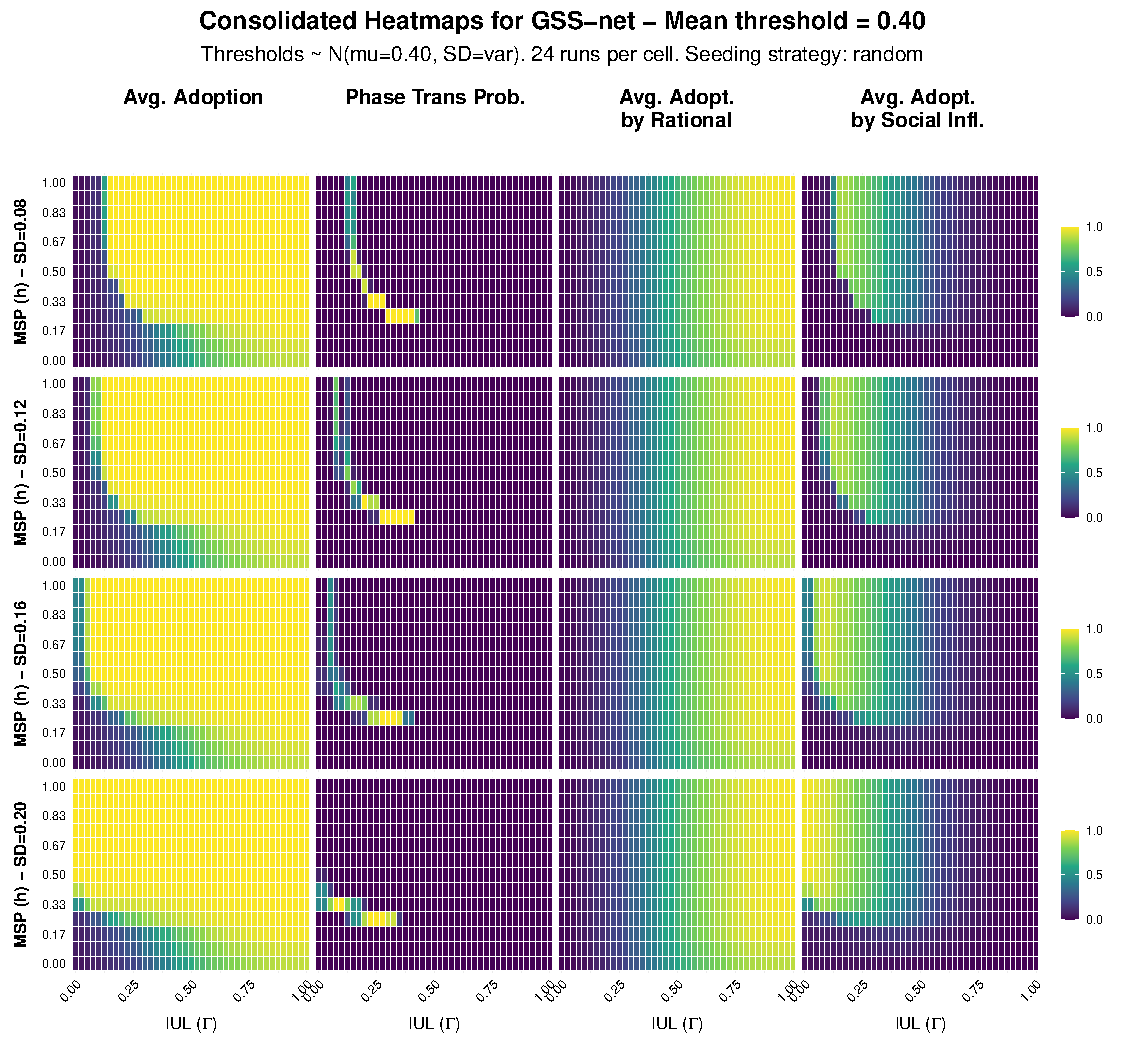
\includegraphics[width=0.8\textwidth]{../figures/plots_m04_random_GSS.pdf}
    \caption{Heatmap of Total Adoption showing phase transitions where adoption jumps from low to high as social flexibility ($h$) increases.}
    \label{fig:heatmap_results}
\end{figure}

Additional surfaces derived from the Generalized Additive Models (BAM) can be found in Appendix \ref{app:surfaces}, further illustrating these non-linear landscapes.

\subsection{Conclusion}
We have demonstrated that adoption is an emergent property of the social structure. By integrating empirical data with a hybrid simulation model, we show that the network topology is a non-neutral scaffold. It actively enables or constrains the potential for social change. In a homophilic world, "who we are" is inextricably linked to "who we know", and our results suggest it is the latter that often casts the deciding vote.

\bibliographystyle{plainnat}
\bibliography{bibliography}

\appendix
\section{Appendix}

\subsection{Network Statistics}
\label{app:net_stats}
Here we show the structural properties of our imputed "Plausible" networks compared to baselines. The clustering coefficients ($C(k)$) and degree distributions confirms the presence of realistic social structure.

\begin{figure}[H]
    \centering
    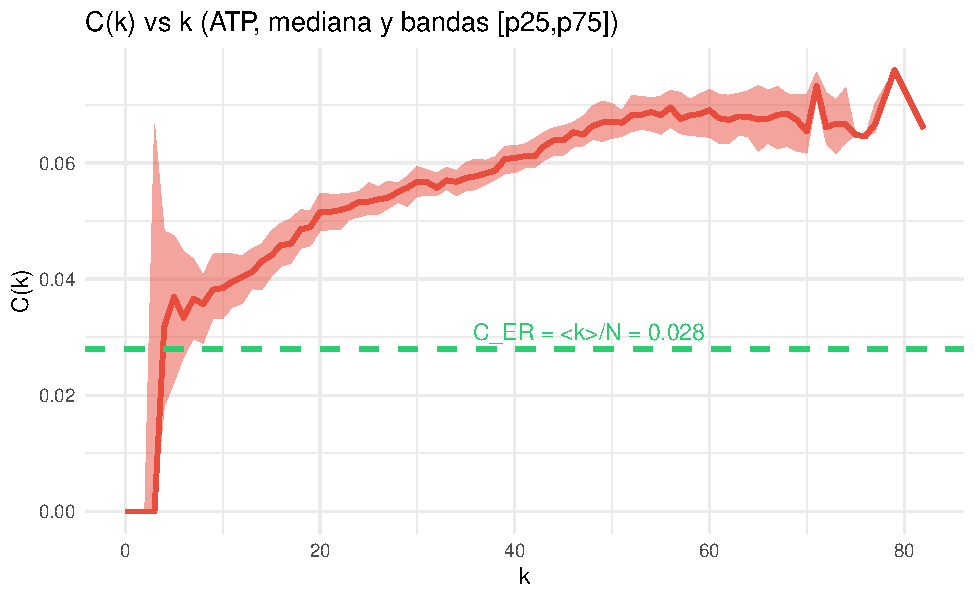
\includegraphics[width=0.48\textwidth]{../figures/ATP_Ck_vs_k.pdf}
    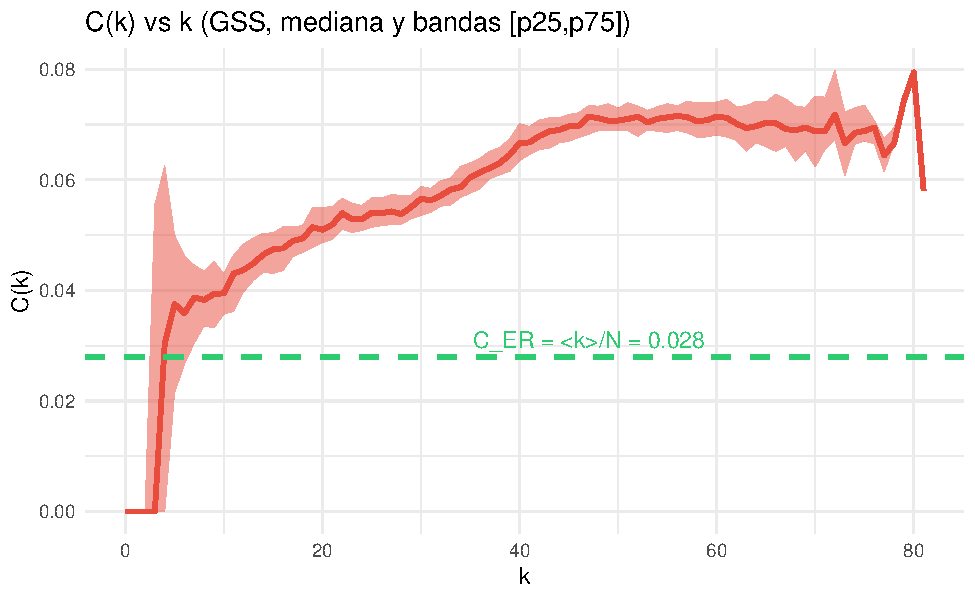
\includegraphics[width=0.48\textwidth]{../figures/GSS_Ck_vs_k.pdf}
    \caption{Clustering Coefficient ($C(k)$) vs Degree ($k$) for ATP (left) and GSS (right) networks.}
    \label{fig:network_stats}
\end{figure}

\begin{figure}[H]
    \centering
    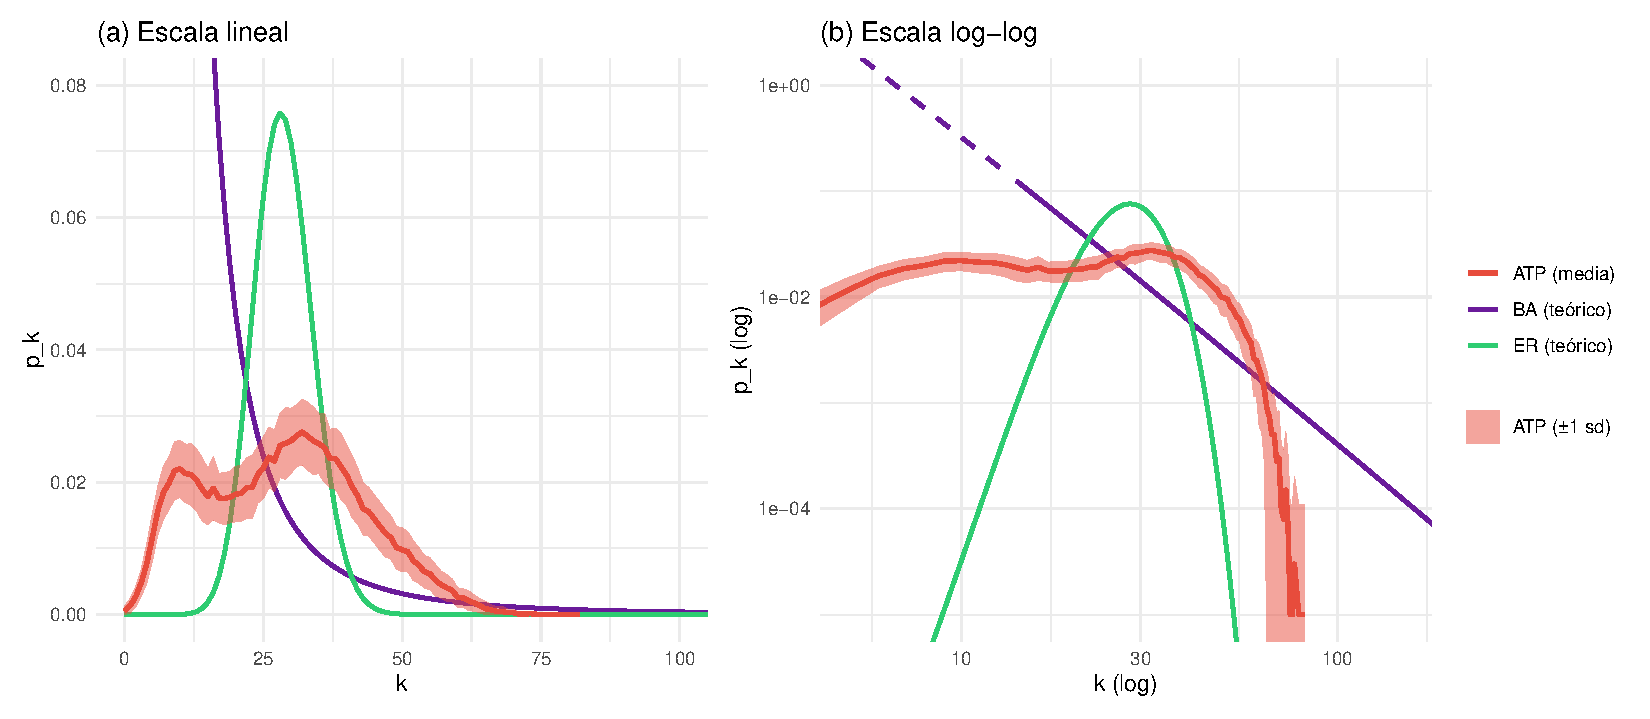
\includegraphics[width=0.48\textwidth]{../figures/ATP_degree_dist.pdf}
    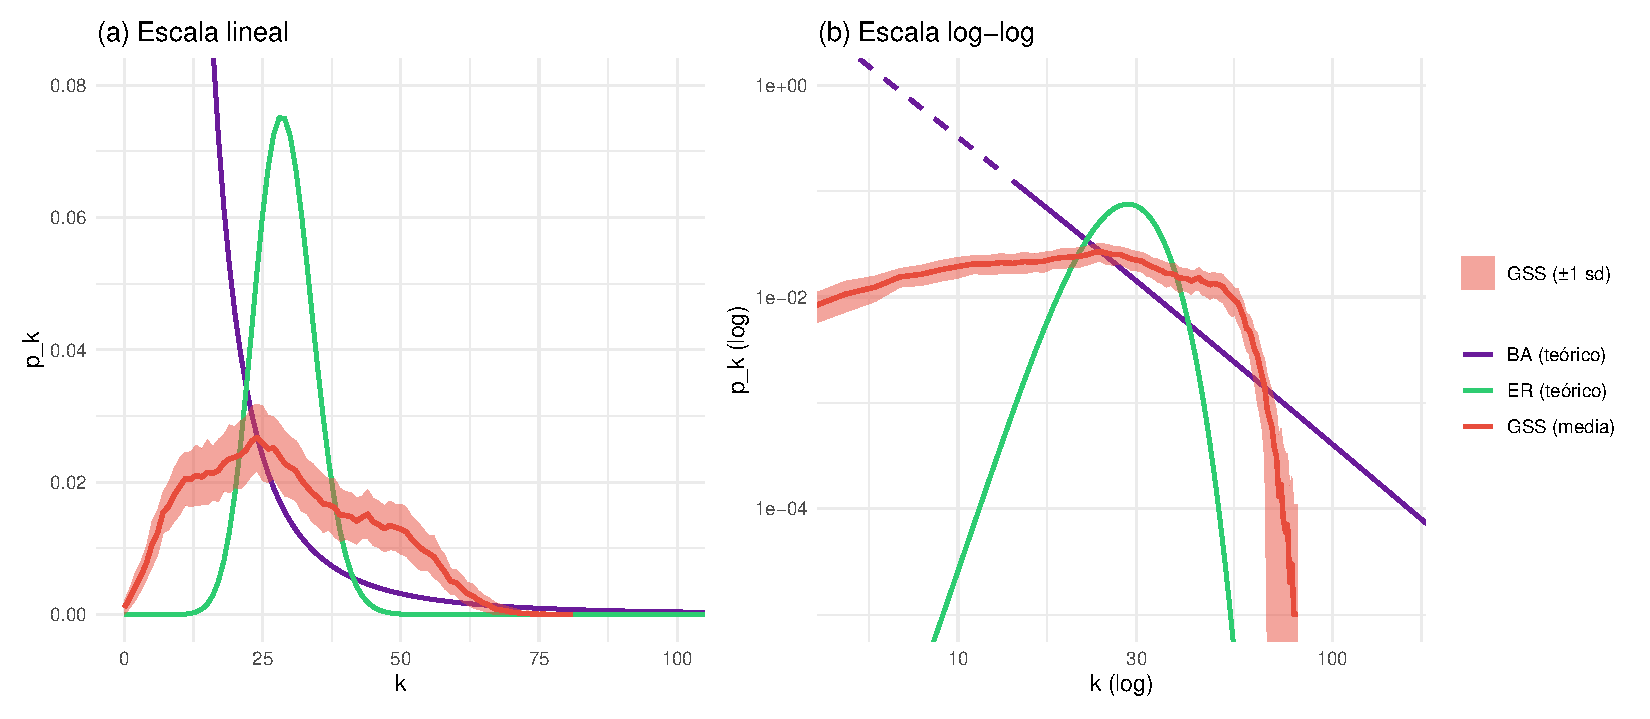
\includegraphics[width=0.48\textwidth]{../figures/GSS_degree_dist.pdf}
    \caption{Degree distributions (log-log scale) for ATP (left) and GSS (right) networks.}
    \label{fig:degree_dist}
\end{figure}


\subsection{Distributions of Minimum Utility Requirements}
\label{app:mur}
\begin{figure}[H]
    \centering
    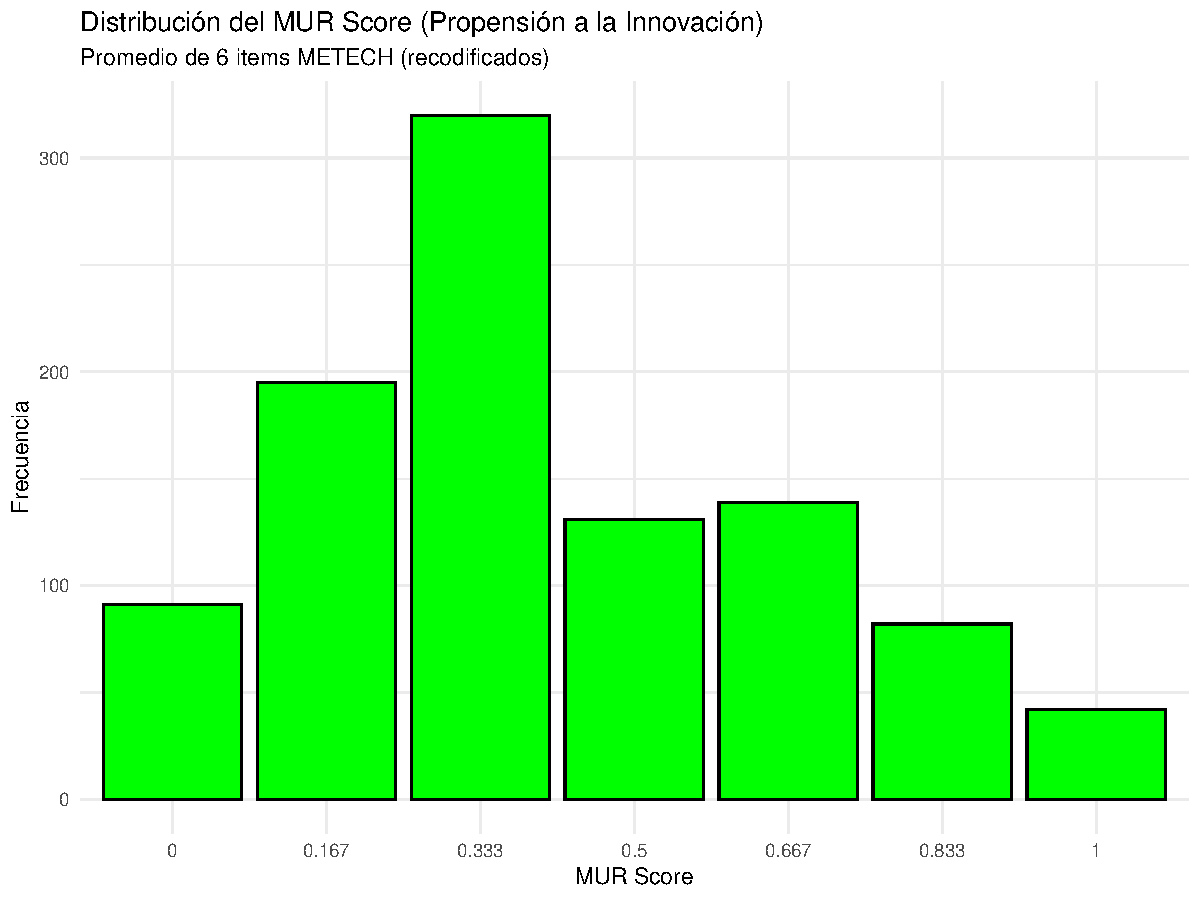
\includegraphics[width=0.38\textwidth]{../figures/ATP_mur_score_distribution.pdf}
    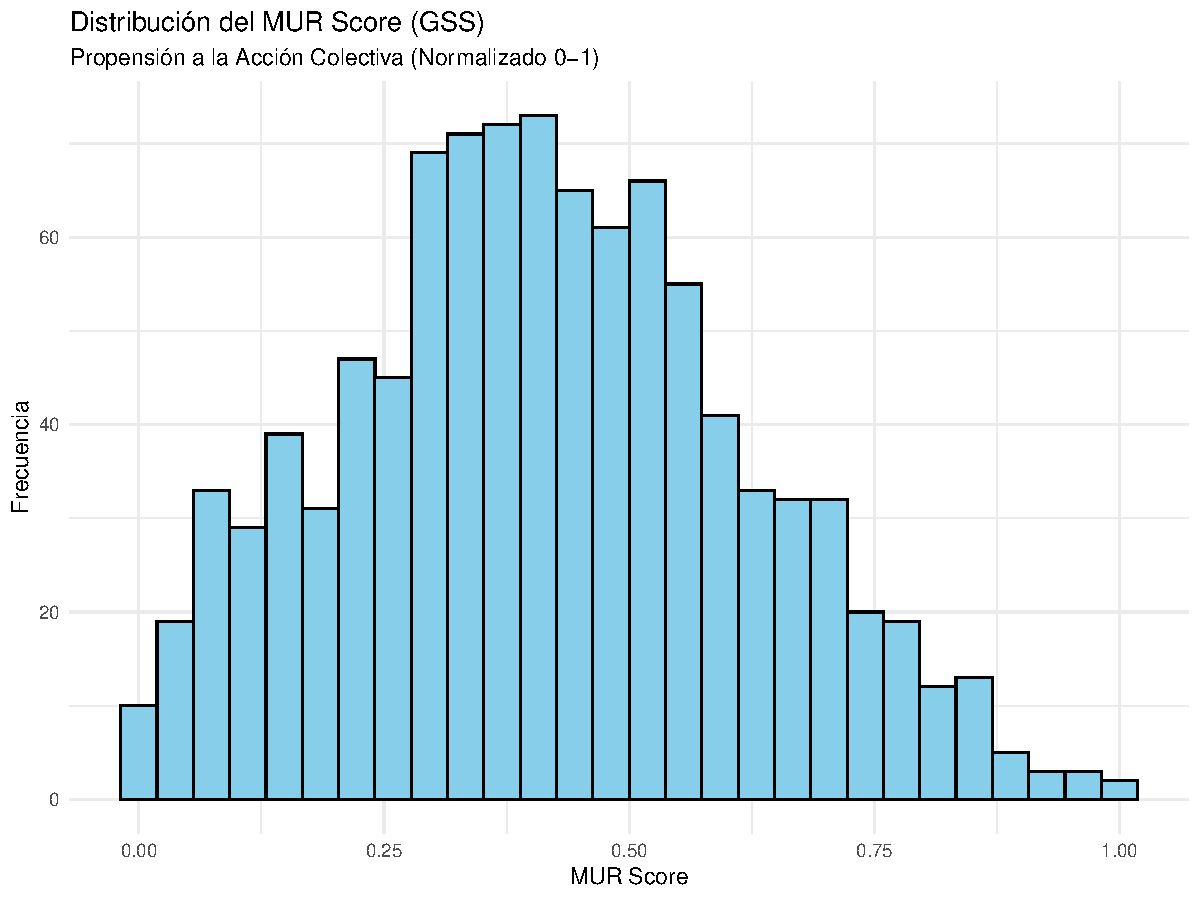
\includegraphics[width=0.38\textwidth]{../figures/GSS_mur_score_distribution.pdf}
    \caption{Distributions of the Minimum Utility Requirement (MUR) derived from "Openness to Innovation" (ATP) and "Propensity to Collective Action" (GSS).}
    \label{fig:mur_dist}
\end{figure}

\subsection{BAM Regression Surfaces}
\label{app:surfaces}
The non-linear surfaces estimated by the Generalized Additive Models show the interaction between Intrinsic Utility Level (IUL) and Maximum Social Proximity (MSP).

\begin{figure}[H]
    \centering
    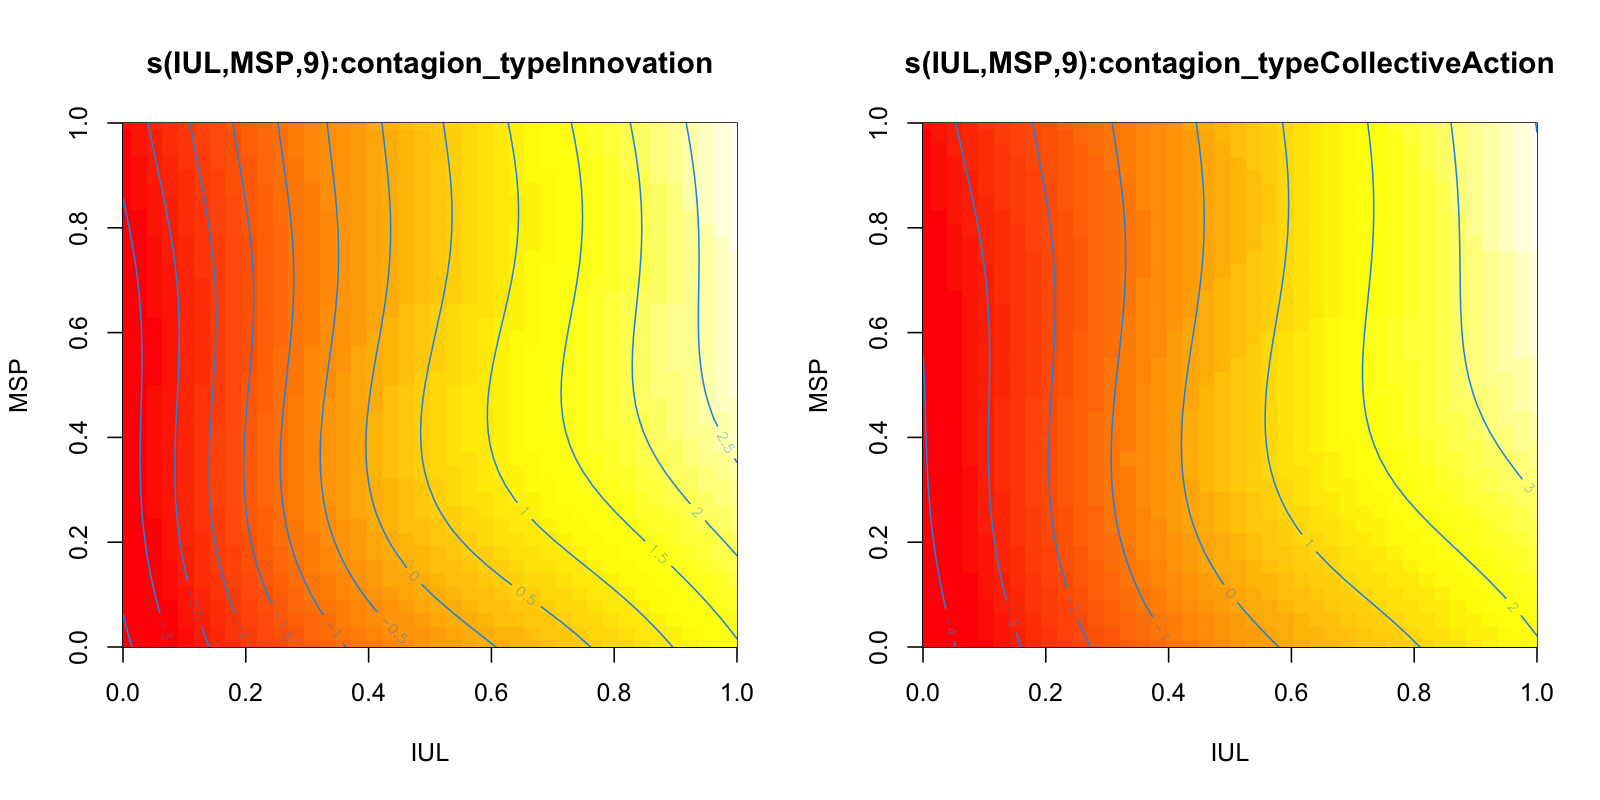
\includegraphics[width=0.32\textwidth]{../figures/bam_rational_surfaces.png}
    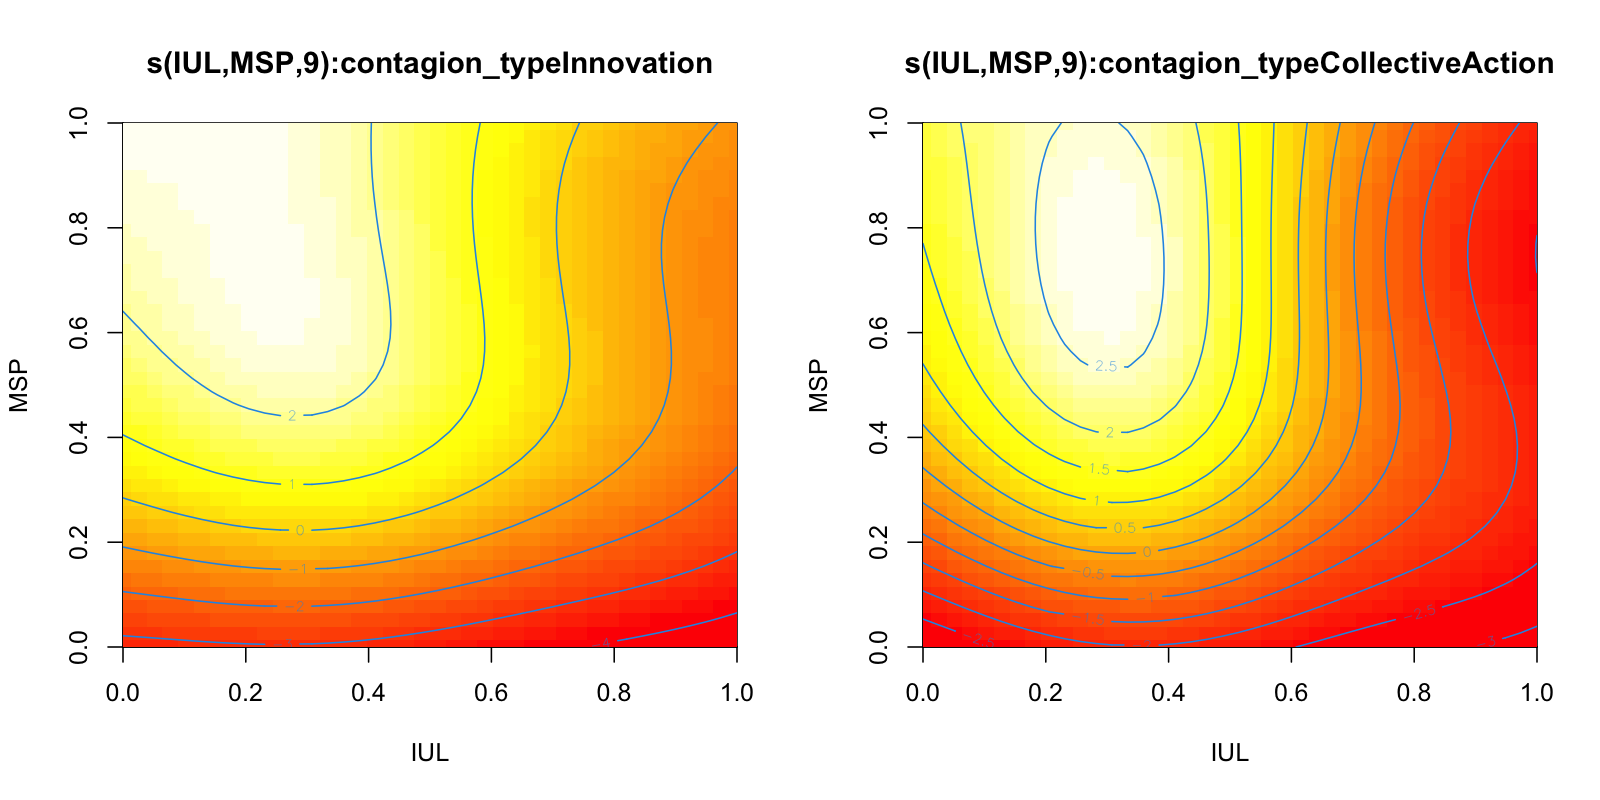
\includegraphics[width=0.32\textwidth]{../figures/bam_social_surfaces.png}
    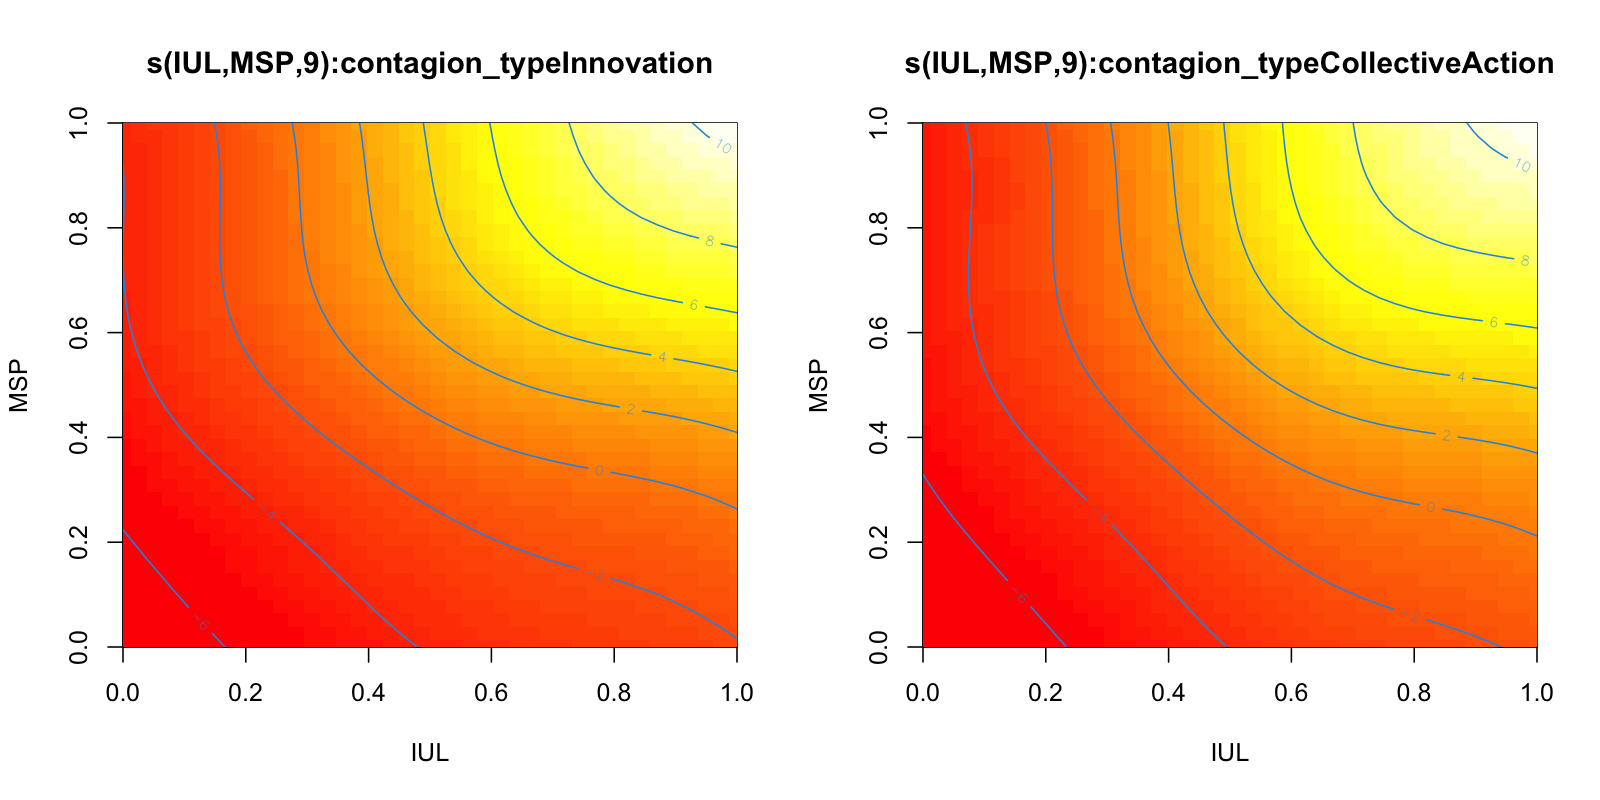
\includegraphics[width=0.32\textwidth]{../figures/bam_total_surfaces.png}
    \caption{Estimated adoption surfaces for Rational (left), Social (center), and Total (right) adoption.}
    \label{fig:bam_surfaces}
\end{figure}

\end{document}
